\documentclass[11pt]{article}

\usepackage{acl2013}
\usepackage{times}
\usepackage{latexsym}
\usepackage{amsmath}
\usepackage{multirow}
\usepackage{array}
\usepackage{url}
\usepackage{graphicx}
\usepackage{subfig}
\usepackage{marvosym}
\usepackage{todonotes}

\setlength\titlebox{6.5cm}

\newcommand{\mnote}[1]{\marginpar{%
  \vskip-\baselineskip
  \raggedright\footnotesize
  \itshape\hrule\smallskip\footnotesize{#1}\par\smallskip\hrule}}

%% \newcommand{\aff}{\ensuremath{{}^\text{\Radioactivity}}}
%% \newcommand{\afff}{\ensuremath{{}^\text{\Bat}}}
\newcommand{\aff}{\ensuremath{{}^\text{1}}}
\newcommand{\afff}{\ensuremath{{}^\text{2}}}
\newcommand{\grammarrule}[3]{$#1 \to \langle \text{#2} , \text{#3} \rangle$ }

\title{Joshua 4.0: Packing, PRO, and Paraphrases}

\author{Juri Ganitkevitch\aff, Yuan Cao\aff, Jonathan Weese\aff, Matt
  Post\afff, and Chris
  Callison-Burch\aff \\
  \aff Center for Language and Speech Processing \\
  \afff Human Language Technology Center of Excellence \\
  Johns Hopkins University}

\date{}

\begin{document}
\maketitle

\begin{abstract}
  We present Joshua 4.0, the newest version of our open-source decoder
  for parsing-based statistical machine translation. The main
  contributions in this release are the introduction of a compact
  grammar representation based on packed tries, and the integration of
  our implementation of pairwise ranking optimization, J-PRO. We
  further present the extension of the Thrax SCFG grammar extractor to
  pivot-based extraction of syntactically informed sentential
  paraphrases.
\end{abstract}

\section{Introduction}
\label{sec-intro}

Joshua is an open-source toolkit\footnote{\url{joshua-decoder.org}}
for parsing-based statistical machine translation of human
languages. The original version of Joshua \cite{Joshua-WMT} was a
reimplementation of the Python-based Hiero machine translation system
\cite{Chiang2007}. It was later extended to support grammars with rich
syntactic labels \cite{li2010joshua}. More recent efforts introduced
the Thrax module, an extensible Hadoop-based extraction toolkit for
synchronous context-free grammars \cite{Joshua-3.0}.

In this paper we describe a set of recent extensions to the Joshua
system. We present a new compact grammar representation format that
leverages sparse features, quantization, and data redundancies to
store grammars in a dense binary format. This allows for both
near-instantaneous start-up times and decoding with extremely large
grammars. In Section~\ref{sec-compact-grammar} we outline our packed
grammar format and present experimental results regarding its impact
on decoding speed, memory use and translation quality.

Additionally, we present Joshua's implementation of the pairwise
ranking optimization \cite{PRO2011} approach to translation model
tuning. J-PRO, like Z-MERT, makes it easy to implement new metrics and
comes with both a built-in perceptron classifier and out-of-the-box
support for widely used binary classifiers such as MegaM and
MaxEnt \cite{MegaM,MaxEnt}. We describe our implementation in
Section~\ref{sec-pro}, presenting experimental results on performance,
classifier convergence, and tuning speed.

Finally, we introduce the inclusion of bilingual pivoting-based
paraphrase extraction into Thrax, Joshua's grammar extractor. Thrax's
paraphrase extraction mode is simple to use, and yields
state-of-the-art syntactically informed sentential paraphrases
\cite{Ganitkevitch2011}. The full feature set of Thrax
\cite{Joshua-3.0} is supported for paraphrase grammars. An easily
configured feature-level pruning mechanism allows to keep the
paraphrase grammar size manageable. Section~\ref{sec-thrax} presents
details on our paraphrase extraction module.

\section{Compact Grammar Representation}
\label{sec-compact-grammar}

Statistical machine translation systems tend to perform better when
trained on larger amounts of bilingual parallel data. Using tools such
as Thrax, translation models and their parameters are extracted and
estimated from the data. In Joshua, translation models are represented
as synchronous context-free grammars (SCFGs). An SCFG is a collection
of rules $\{\mathbf{r}_i\}$ that take the form:
\begin{equation}
 \mathbf{r}_i = C_i \to \langle \alpha_i , \gamma_i , \sim_i, \vec{\varphi}_i \rangle ,
\end{equation}
where \emph{left-hand side} $C_i$ is a nonterminal symbol, the
\emph{source side} $\alpha_i$ and the \emph{target side} $\gamma_i$
are sequences of both nonterminal and terminal symbols. Further,
$\sim_i$ is a one-to-one correspondence between the nonterminal
symbols of $\alpha_i$ and $\gamma_i$, and $\vec{\varphi}_i$ is a
vector of features quantifying the probability of $\alpha_i$
translating to $\gamma_i$, as well as other characteristics of the
rule \cite{Joshua-3.0}. At decoding time, Joshua loads the grammar
rules into memory in their entirety, and stores them in a trie data
structure indexed by the rules' source side. This allows the decoder
to efficiently look up rules that are applicable to a particular span
of the (partially translated) input.

As the size of the training corpus grows, so does the resulting
translation grammar. Using more diverse sets of nonterminal labels --
which can significantly improve translation performance -- further
aggravates this problem. As a consequence, the space requirements for
storing the grammar in memory during decoding quickly grow
impractical. In some cases grammars may become too large to fit into
the memory on a single machine.

As an alternative to the commonly used trie structures based on hash
maps, we propose a packed trie representation for SCFGs. The approach
we take is similar to work on efficiently storing large phrase tables
by \newcite{Zens2007} and language models by \newcite{KenLM} and
\newcite{BerkeleyLM} -- both language model implementations are now
integrated with Joshua.

\subsection{Packed Synchronous Tries}

For our grammar representation, we break the SCFG up into three
distinct structures. As Figure~\ref{fig-packed-structure} indicates,
we store the grammar rules' source sides $\{\alpha_i\}$, target sides
$\{\gamma_i\}$, and feature data $\{\vec{\varphi}_i\}$ in separate
formats of their own. Each of the structures is packed into a flat
array, and can thus be quickly read into memory. All terminal and
nonterminal symbols in the grammar are mapped to integer symbol id's
using a globally accessible vocabulary map. We will now describe the
implementation details for each representation and their interactions
in turn.

\begin{figure*}[!th]
\begin{center}
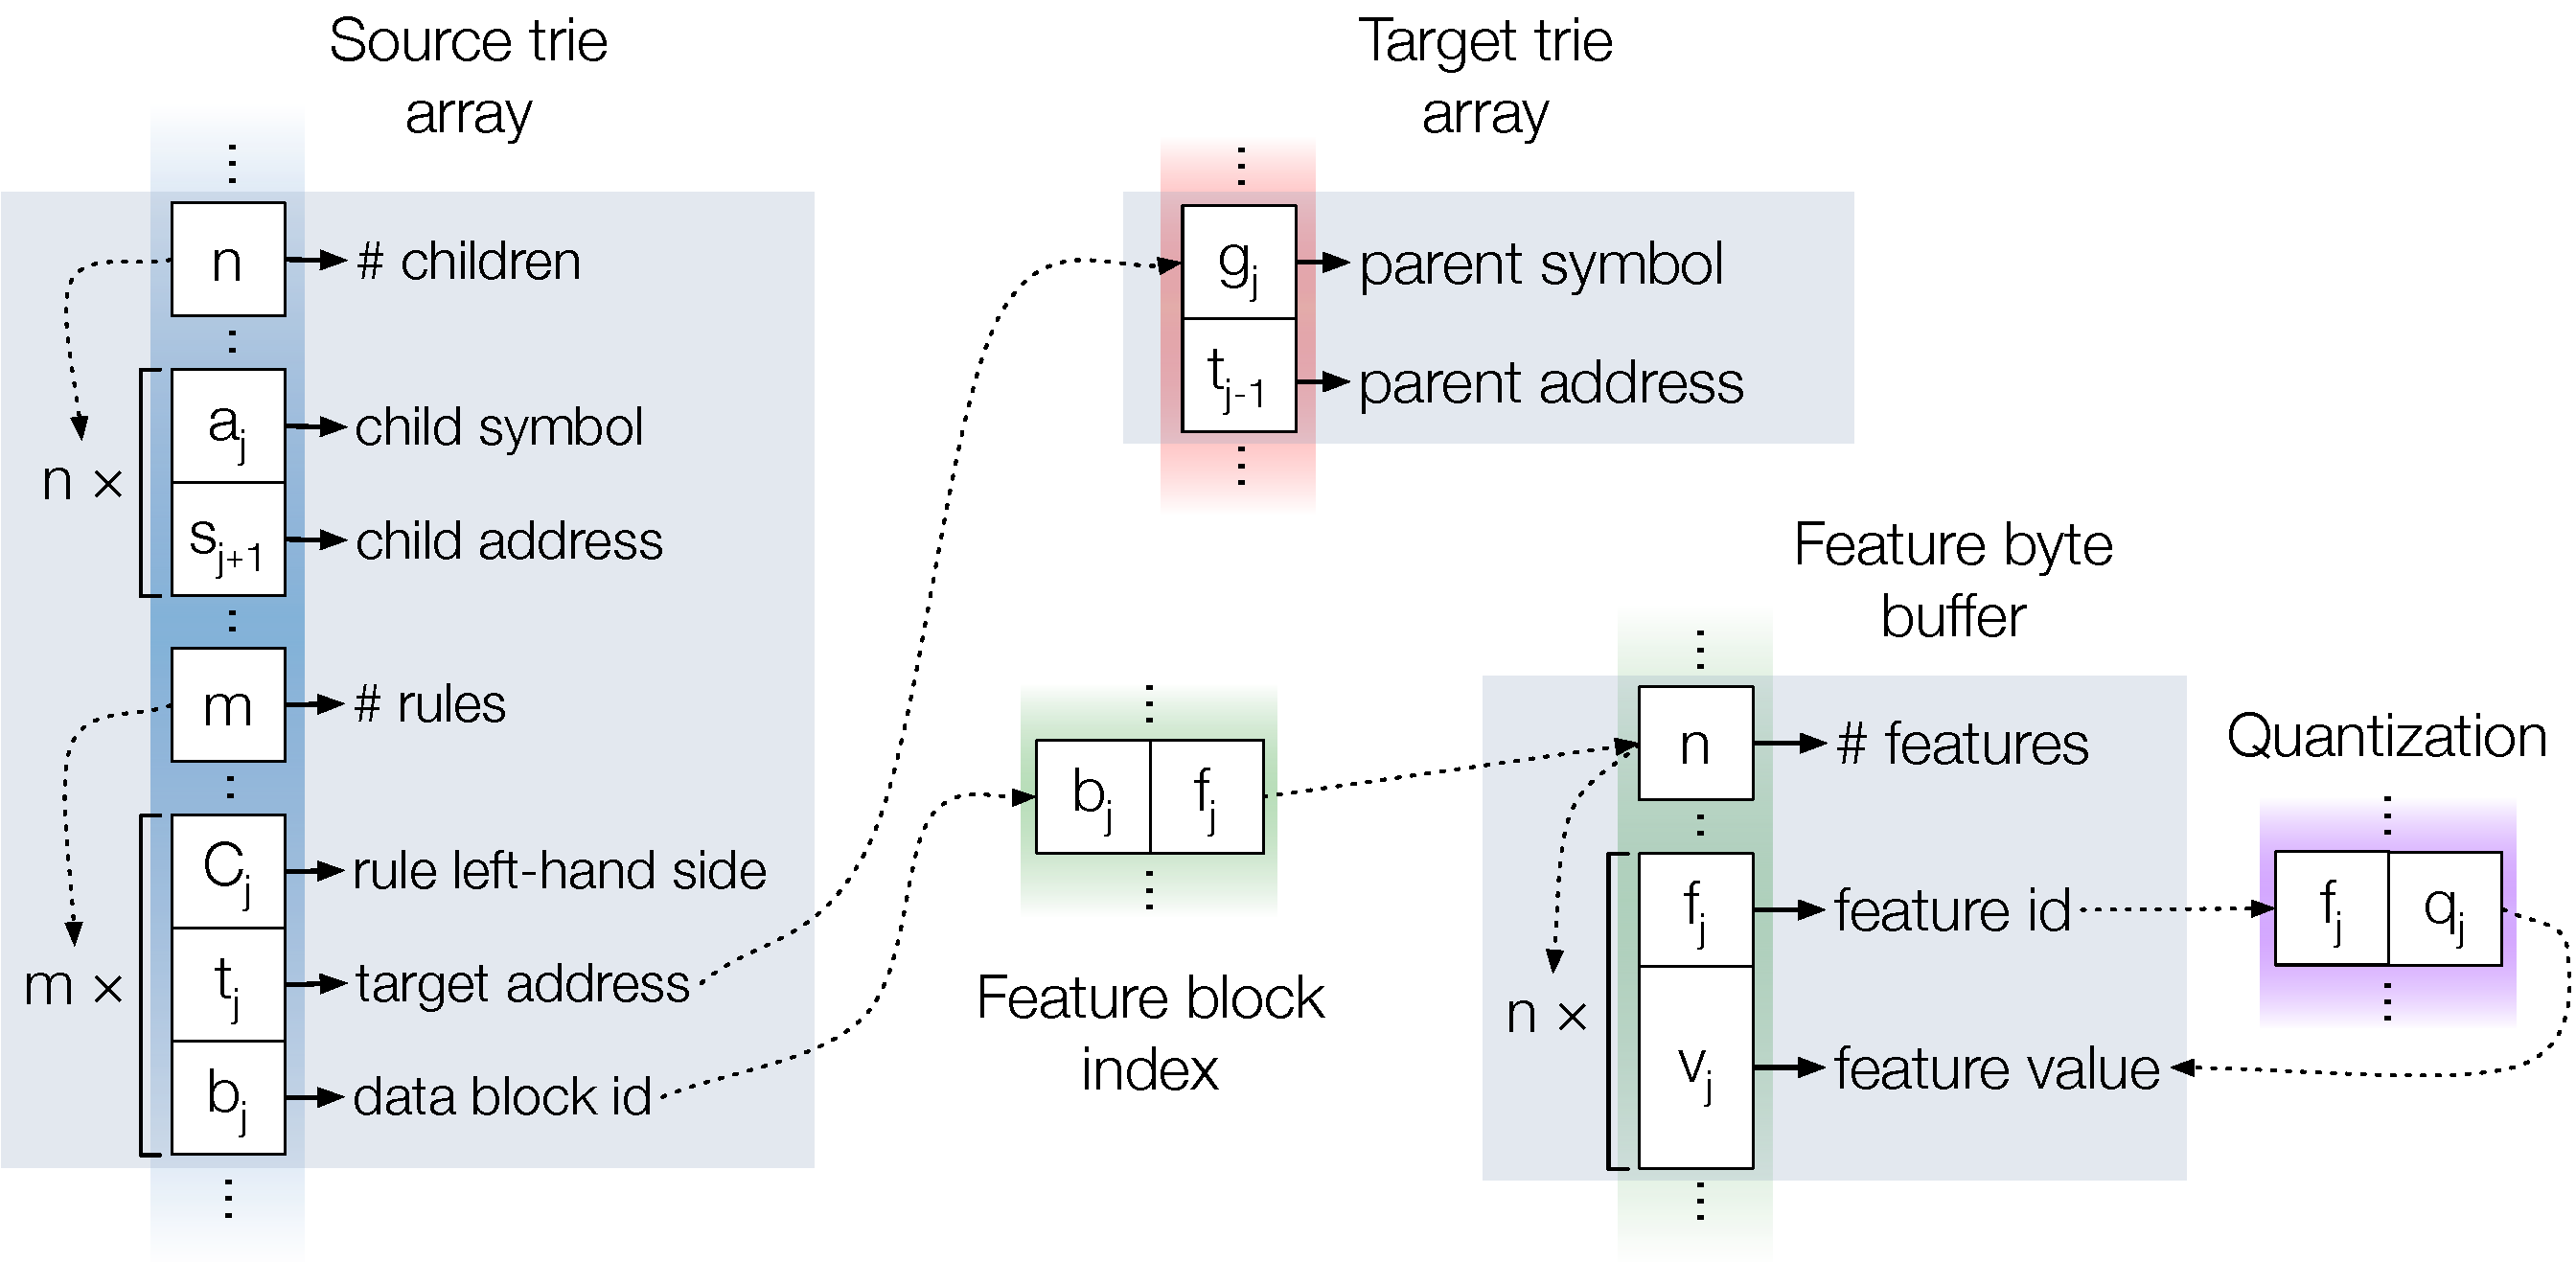
\includegraphics[width=0.9\linewidth]{figures/packed_structure.pdf}
\end{center}
\caption{An illustration of our packed grammar data structures. The
  source sides of the grammar rules are stored in a packed trie. Each
  node may contain $n$ children and the symbols linking to them, and
  $m$ entries for rules that share the same source side. Each rule
  entry links to a node in the target-side trie, where the full target
  string can be retrieved by walking up the trie until the root is
  reached. The rule entries also contain a data block id, which
  identifies feature data attached to the rule. The features are
  encoded according to a type/quantization specification and stored as
  variable-length blocks of data in a byte buffer.}
\label{fig-packed-structure}
\end{figure*}

\subsubsection{Source-Side Trie}

The source-side trie (or source trie) is designed to facilitate
efficient lookup of grammar rules by source side, and to allow us to
completely specify a matching set of rule with a single integer index
into the trie. We store the source sides $\{\alpha_i\}$ of a grammar
in a downward-linking trie, i.e. each trie node maintains a record of
its children. The trie is packed into an array of 32-bit
integers. Figure~\ref{fig-packed-structure} illustrates the
composition of a node in the source-side trie. All information
regarding the node is stored in a contiguous block of integers, and
decomposes into two parts: a \emph{linking block} and a \emph{rule
  block}.

The linking block stores the links to the child trie nodes. It
consists of an integer $n$, the number of children, and $n$ blocks of
two integers each, containing the symbol id $a_j$ leading to the child
and the child node's address $s_j$ (as an index into the source-side
array). The children in the link block are sorted by symbol id,
allowing for a lookup via binary or interpolation search.

The rule block stores all information necessary to reconstruct the
rules that share the source side that led to the current source trie
node. It stores the number of rules, $m$, and then a tuple of three
integers for each of the $m$ rules: we store the symbol id of the
left-hand side, an index into the target-side trie and a \emph{data
  block id}. The rules in the data block are initially in an arbitrary
order, but are sorted by application cost upon loading.

\subsubsection{Target-Side Trie}

The target-side trie (or target trie) is designed to enable us to
uniquely identify a target side $\gamma_i$ with a single pointer into
the trie, as well as to exploit redundancies in the target side
string. Like the source trie, it is stored as an array of
integers. However, the target trie is a \emph{reversed}, or
upward-linking trie: a trie node retains a link to its parent, as well
as the symbol id labeling said link.

As illustrated in Figure~\ref{fig-packed-structure}, the target trie
is accessed by reading an array index from the source trie, pointing
to a trie node at depth $d$. We then follow the parent links to the
trie root, accumulating target side symbols $g_j$ into a target side
string $g_1^d$ as we go along. In order to match this traversal, the
target strings are entered into the trie in reverse order, i.e. last
word first. In order to determine $d$ from a pointer into the target
trie, we maintain an offset table in which we keep track of where each
new trie level begins in the array. By first searching the offset
table, we can determine $d$, and thus know how much space to allocate
for the complete target side string.

To further benefit from the overlap there may be among the target
sides in the grammar, we drop the nonterminal labels from the target
string prior to inserting them into the trie. For richly labeled
grammars, this collapses all lexically identical target sides that
share the same nonterminal reordering behavior, but vary in
nonterminal labels into a single path in the trie. Since the
nonterminal labels are retained in the rules' source sides, we do not
lose any information by doing this.


\subsubsection{Features and Other Data}

We designed the data format for the grammar rules' feature values to
be easily extended to include other information that we may want to
attach to a rule, such as word alignments, or locations of occurrences
in the training data. In order to that, each rule $\mathbf{r}_i$ has a
unique block id $b_i$ associated with it. This block id identifies the
information associated with the rule in every attached data store. All
data stores are implemented as memory-mapped byte buffers that are
only loaded into memory when actually requested by the decoder. The
format for the feature data is detailed in the following.

The rules' feature values are stored as sparse features in contiguous
blocks of variable length in a byte buffer. As shown in
Figure~\ref{fig-packed-structure}, a lookup table is used to map the
$b_i$ to the index of the block in the buffer. Each block is
structured as follows: a single integer, $n$, for the number of
features, followed by $n$ feature entries. Each feature entry is led
by an integer for the feature id $f_j$, and followed by a field of
variable length for the feature value $v_j$. The size of the value is
determined by the type of the feature. Joshua maintains a quantization
configuration which maps each feature id to a type handler or
\emph{quantizer}. After reading a feature id from the byte buffer, we
retrieve the responsible quantizer and use it to read the value from
the byte buffer.

Joshua's packed grammar format supports Java's standard primitive
types, as well as an 8-bit quantizer. We chose 8 bit as a compromise
between compression, value decoding speed and translation performance
\cite{Federico2006}. Our quantization approach follows
\newcite{Federico2006} and \newcite{KenLM} in partitioning the value
histogram into 256 equal-sized buckets. We quantize by mapping each
feature value onto the weighted average of its bucket. Joshua allows
for an easily per-feature specification of type. Quantizers can be
share statistics across multiple features with similar value
distributions.


\subsection{Experiments}

\begin{table}[!t]
\centering
\begin{tabular}{|l|c|c|}
  \hline
  Grammar & Format & Memory \\
  \hline\hline
  \multirow{2}{*}{Hiero (43M rules)} & Baseline & 13.6G \\
  & Packed & 1.8G \\
  \hline
  \hline
  \multirow{2}{*}{Syntax (200M rules)} & Baseline & 99.5G \\
  &  Packed & 9.8G \\
  &  Packed 8-bit & 5.8G \\
  \hline
\end{tabular}
\caption{Decoding-time memory use for the packed grammar
  versus the standard grammar format. Even without lossy quantization the
  packed grammar representation yields significant savings in memory
  consumption. Adding 8-bit quantization for the real-valued features
  in the grammar reduces even large syntactic grammars to a manageable
  size.}
\label{tab-memory}
\end{table}

We assess the packed grammar representation's memory efficiency and
impact on the decoding speed on the WMT12 French-English
task. Table~\ref{tab-memory} shows a comparison of the memory needed
to store our WMT12 French-English grammars at runtime. We can observe
a substantial decrease in memory consumption for both Hiero-style
grammars and the much larger syntactically annotated grammars. Even
without any feature value quantization, the packed format achieves an
80\% reduction in space requirements. Adding 8-bit quantization for
the log-probability features yields even smaller grammar sizes, in
this case a reduction of over 94\%.

\begin{figure}[!t]
  \begin{center}
    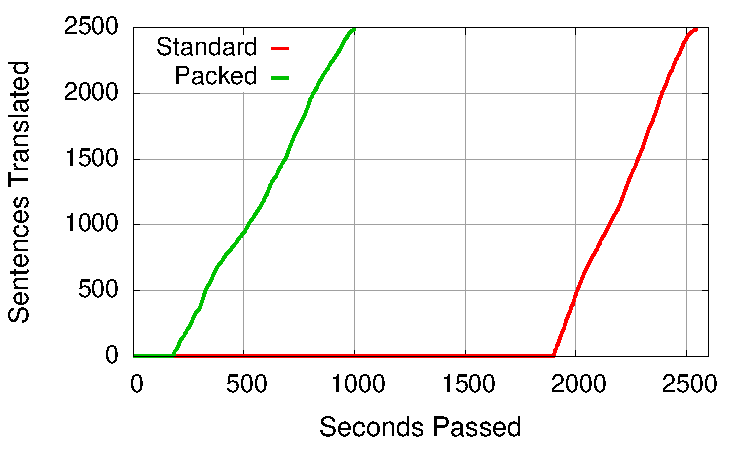
\includegraphics[width=0.99\linewidth]{figures/progress.pdf}
  \end{center}
  \label{fig:speed}
  \caption{A visualization of the loading and decoding speed on the
    WMT12 French-English development set contrasting the packed
    grammar representation with the standard format. Grammar loading
    for the packed grammar representation is substantially faster than
    that for the baseline setup. Even with a slightly slower decoding
    speed (note the difference in the slopes) the packed grammar
    finishes in less than half the time, compared to the standard
    format.}
\end{figure}

In order to avoid costly repeated retrievals of individual feature
values of rules, we compute and cache the stateless application cost
for each grammar rule at grammar loading time. This, alongside with a
lazy approach to rule lookup allows us to largely avoid losses in
decoding speed.

Figure~\label{fig:speed} shows a translation progress graph for the
WMT12 French-English development set. Both systems load a Hiero-style
grammar with 43 million rules, and use 16 threads for parallel
decoding. The initial loading time for the packed grammar
representation is dramatically shorter than that for the baseline
setup (a total of 176 seconds for loading and sorting the grammar,
versus 1897 for the standard format). Even though decoding speed is
slightly slower with the packed grammars (an average of 5.3 seconds
per sentence versus 4.2 for the baseline), the effective translation
speed is more than twice that of the baseline (1004 seconds to
complete decoding the 2489 sentences, versus 2551 seconds with the
standard setup).


\section{J-PRO: Pairwise Ranking Optimization in Joshua}
\label{sec-pro}

Pairwise ranking optimization (PRO) proposed by \cite{PRO2011} is
a new method for discriminative parameter tuning in statistical
machine translation. It is reported to be more stable than the popular
MERT algorithm \cite{Och2003} and is more scalable with regard to the
number of features. PRO treats parameter tuning as an $n$-best list
reranking problem, and the idea is similar to other pairwise ranking
techniques like ranking SVM and IR SVMs \cite{Hang2011}. The algorithm
can be described thusly:

Let $h(c)=\langle \mathbf{w},\mathbf{\Phi}(c)\rangle$ be the linear
model score of a candidate translation $c$, in which
$\mathbf{\Phi}(c)$ is the feature vector of $c$ and $\mathbf{w}$ is
the parameter vector. Also let $g(c)$ be the metric score of $c$
(without loss of generality, we assume a higher score indicates a
better translation). We aim to find a parameter vector $\mathbf{w}$
such that for a pair of candidates $\{ c_i,c_j \}$ in an $n$-best
list,
\begin{align*}
  (h(c_i)-h(c_j))(g(c_i)-g(c_j)) & = \\
  & \hspace{-120pt} \langle \mathbf{w},\mathbf{\Phi}(c_i) -
  \mathbf{\Phi}(c_j)\rangle (g(c_i)-g(c_j)) >0 ,
\end{align*}
namely the order of the model score is consistent with that of the
metric score. This can be turned into a binary classification problem,
by adding instance
$$\Delta\mathbf{\Phi}_{ij}=\mathbf{\Phi}(c_i) - \mathbf{\Phi}(c_j)$$
with class label $\mathit{sign}(g(c_i)-g(c_j))$ to the training data (and
symmetrically add instance
$$\Delta\mathbf{\Phi}_{ji}=\mathbf{\Phi}(c_j) - \mathbf{\Phi}(c_i)$$
with class label $\mathit{sign}(g(c_j)-g(c_i))$ at the same time),
then using any binary classifier to find the $\mathbf{w}$ which
determines a hyperplane separating the two classes (therefore the
performance of PRO depends on the choice of classifier to a large
extent). Given a training set with $T$ sentences, there are $O(Tn^2)$
pairs of candidates that can be added to the training set, this number
is usually much too large for efficient training. To make the task
more tractable, PRO samples a subset of the candidate pairs so that
only those pairs whose metric score difference is large enough are
qualified as training instances. This follows the intuition that high
score differential makes it easier to separate good translations from
bad ones.

\subsection{Implementation}
\label{sec-jpro}

\begin{figure*}[!t]
  \begin{center}$
    \begin{array}{ccc}
      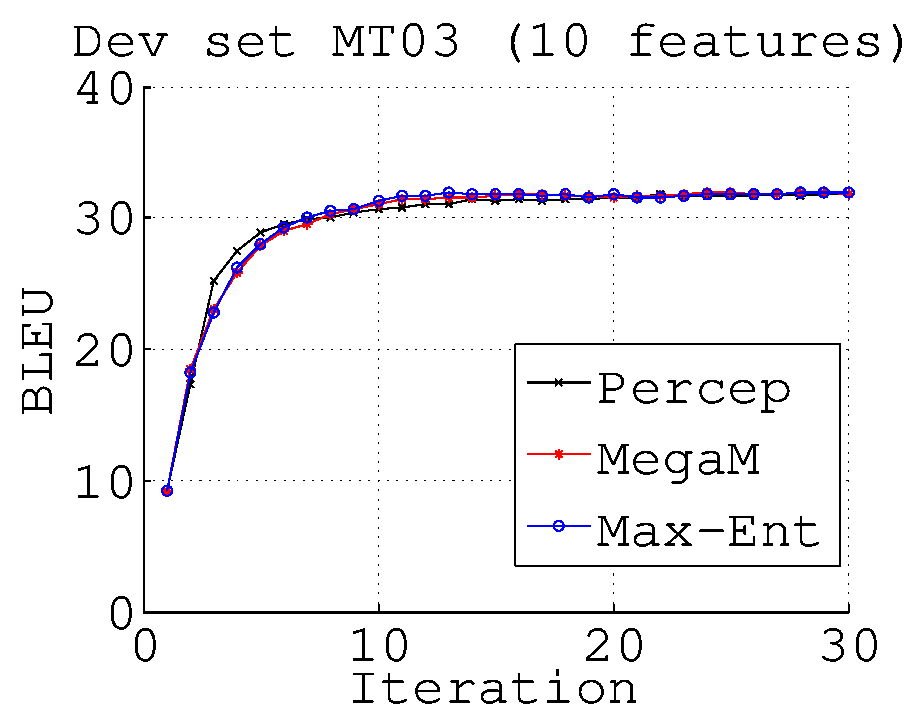
\includegraphics[width=0.3\textwidth]{figures/mt03_10feat.pdf}
      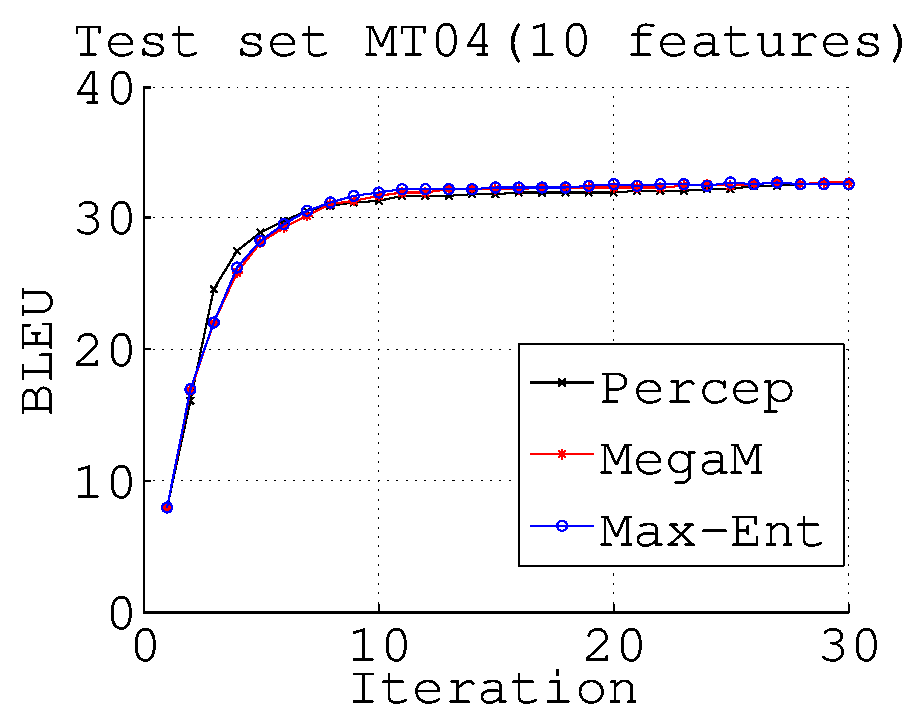
\includegraphics[width=0.3\textwidth]{figures/mt04_10feat.pdf}
      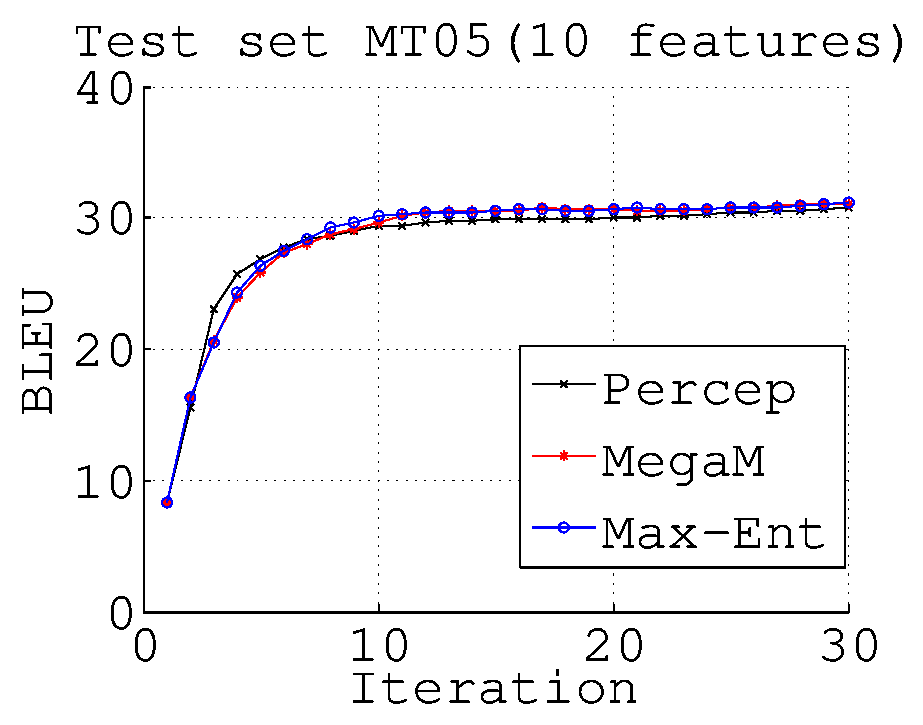
\includegraphics[width=0.3\textwidth]{figures/mt05_10feat.pdf}\\
      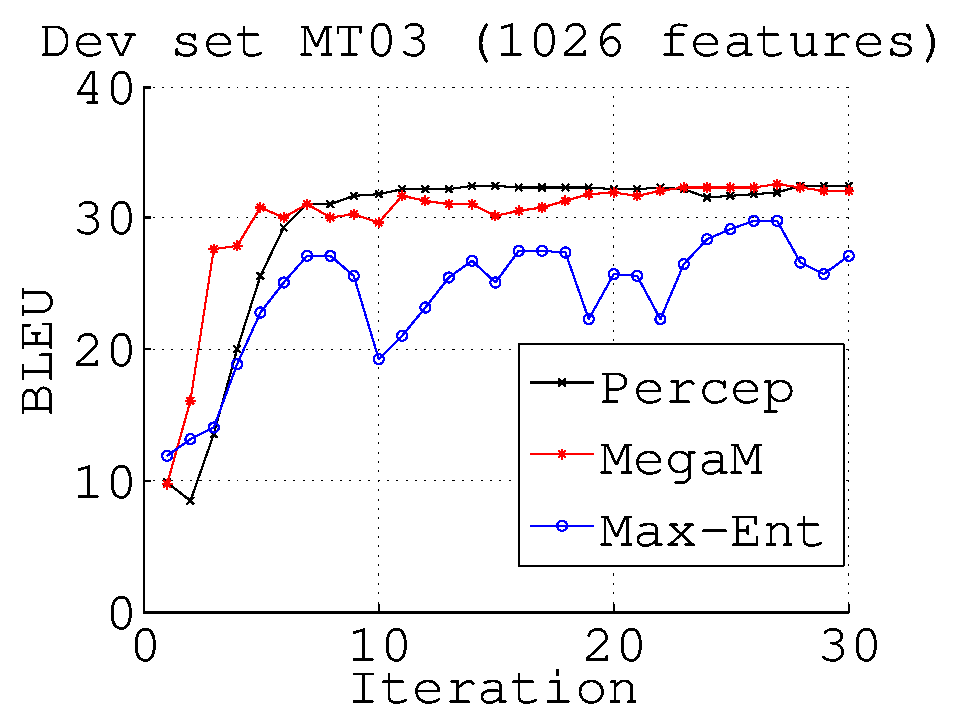
\includegraphics[width=0.3\textwidth]{figures/mt03_1026feat.pdf}
      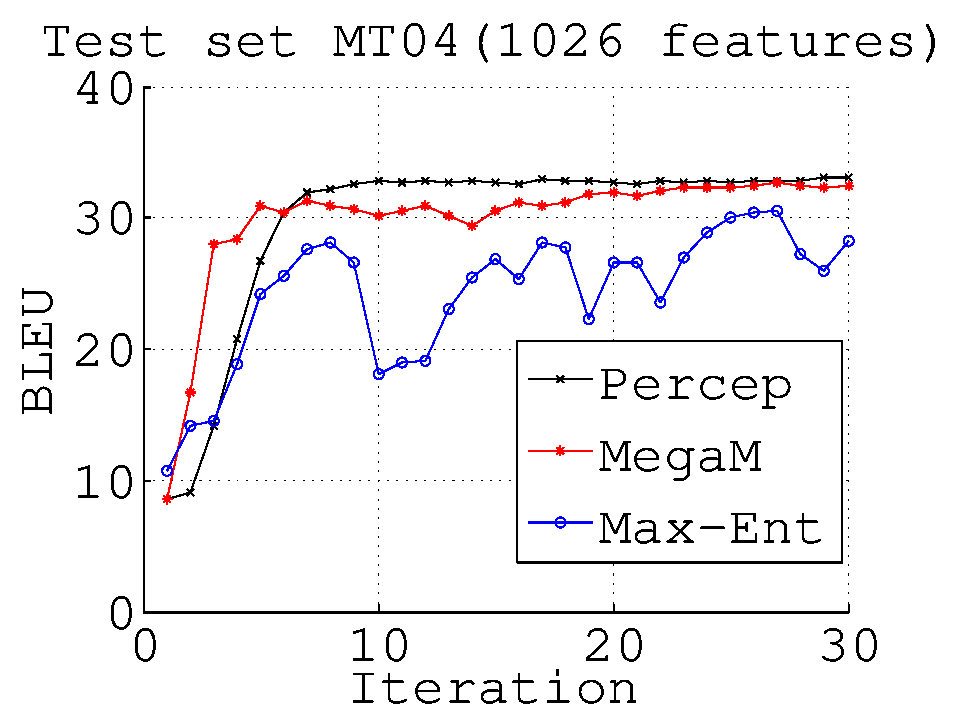
\includegraphics[width=0.3\textwidth]{figures/mt04_1026feat.pdf}
      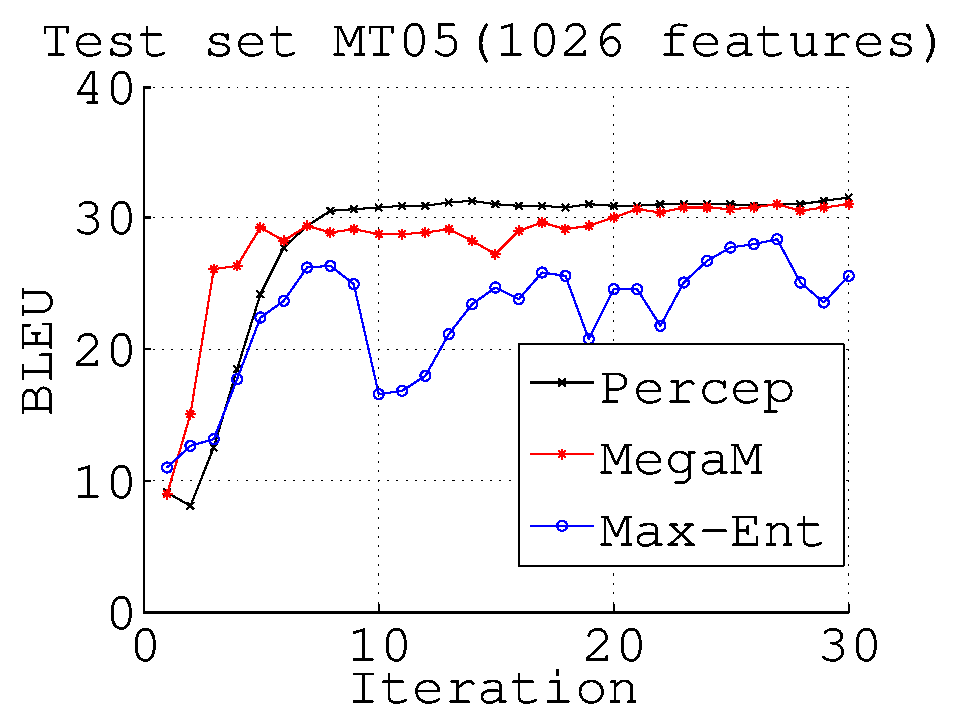
\includegraphics[width=0.3\textwidth]{figures/mt05_1026feat.pdf}
    \end{array}$
  \end{center}
  \caption{\label{fig:pro1}Experimental results on the development and
    test sets. The $x$-axis is the number of iterations (up to 30) and
    the $y$-axis is the BLEU score. The three curves in each figure
    correspond to three classifiers. Upper row: results trained using
    only dense features (10 features); Lower row: results trained
    using dense+sparse features (1026 features). Left column:
    development set (MT03); Middle column: test set (MT04); Right
    column: test set (MT05).}
\end{figure*}

PRO is implemented in Joshua 4.0 named J-PRO. In order to ensure
compatibility with the decoder and the parameter tuning module Z-MERT
\cite{zaidan2009z} included in all versions of Joshua, J-PRO is built
upon the architecture of Z-MERT with similar usage and configuration
files(with a few extra lines specifying PRO-related parameters). J-PRO
inherits Z-MERT's ability to easily plug in new metrics. Since PRO
allows using any off-the-shelf binary classifiers, J-PRO provides a
Java interface that enables easy plug-in of any classifier. Currently,
J-PRO supports three classifiers:
\begin{itemize}
\item \emph{Perceptron} \cite{Rosenblatt1958}: the perceptron is
self-contained in J-PRO, no external resources required.

\item \emph{MegaM} \cite{MegaM}: the classifier used by
\newcite{PRO2011}.\footnote{\url{hal3.name/megam}}

\item \emph{Maximum entropy classifier} \cite{MaxEnt}: the Stanford
  toolkit for maximum entropy classification.\footnote{
    \url{nlp.stanford.edu/software}}
\end{itemize}  
The user may specify which classifier he wants to use and the
classifier-specific parameters in the J-PRO configuration file.

The PRO approach is capable of handling a large number of features,
allowing the use of sparse discriminative features for machine
translation.  However, \newcite{Kristy2008} demonstrated that naively
tuning weights for a heterogeneous feature set composed of both dense
and sparse features can yield subpar results. Thus, to better handle
the relation between dense and sparse features and provide a flexible
selection of training schemes, J-PRO supports the following four
training modes. We assume $M$ dense features and $N$ sparse features
are used:
\begin{enumerate}
\item Tune the dense feature parameters only, just like Z-MERT ($M$
  parameters to tune).
\item Tune the dense + sparse feature parameters together ($M+N$
  parameters to tune).
\item Tune the sparse feature parameters only with the dense feature
  parameters fixed, and sparse feature parameters scaled by a manually
  specified constant ($N$ parameters to tune).
\item Tune the dense feature parameters and the scaling factor for
  sparse features, with the sparse feature parameters fixed ($M$+1
  parameters to tune).
\end{enumerate}
J-PRO supports $n$-best list input with a sparse feature format which
enumerates only the firing features together with their values. This
enables a more compact feature representation when numerous features
are involved in training.

\begin{table*}[!t]
\centering
\begin{tabular}{|c|c|c|c|c|}
  \hline
  \multirow{2}{*}{Datasets} & \multirow{2}{*}{Z-MERT} & \multicolumn{3}{c|}{J-PRO} \\
  &       & Percep & MegaM & Max-Ent\\
  \hline\hline
  Dev (MT03)   &32.2  &31.9  &32.0  &32.0 \\
  Test (MT04)  &32.6  &32.7  &32.7  &32.6 \\
  Test (MT05)  &30.7  &30.9  &31.0  &30.9 \\
  \hline
\end{tabular}
\caption{\label{table:pro} Comparison between the results given by
  Z-MERT and J-PRO (trained with 10 features).}
\end{table*}

\subsection{Experiments}

We did our experiments using J-PRO on the NIST Chinese-English data,
and BLEU score was used as the quality metric for experiments reported
in this section.\footnote{We also experimented with other metrics
  including TER, METEOR and TER-BLEU. Similar trends as reported in
  this section were observed. These results are omitted here due to
  limited space.} The experimental settings are as the following:

\emph{Datasets}: MT03 dataset (998 sentences) as development set for
parameter tuning, MT04 (1788 sentences) and MT05 (1082 sentences) as
test sets.

\emph{Features}: Dense feature set include the 10 regular features
used in the Hiero system; Sparse feature set includes 1016 target-side
rule POS bi-gram features as used in \cite{Li2010coling}.

\emph{Classifiers}: Perceptron, MegaM and Maximum entropy.

\emph{PRO parameters}: $\Gamma=8000$ (number of candidate pairs sampled
uniformly from the $n$-best list), $\alpha=1$ (sample acceptance
probability), $\Xi=50$ (number of top candidates to be added to the
training set).

Figure~\ref{fig:pro1} shows the BLEU score curves on the development
and test sets as a function of iterations. The upper and lower rows
correspond to the results trained with 10 dense features and 1026
dense+sparse features respectively. We intentionally selected very bad
initial parameter vectors to verify the robustness of the
algorithm. It can be seen that with each iteration, the BLEU score
increases monotonically on both development and test sets, and begins
to converge after a few iterations. When only 10 features are
involved, all classifiers give almost the same performance. However,
when scaled to over a thousand features, the maximum entropy
classifier becomes unstable and the curve fluctuates significantly. In
this situation MegaM behaves well, but the J-PRO built-in perceptron
gives the most robust performance.

Table~\ref{table:pro} compares the results of running Z-MERT and
J-PRO. Since MERT is not able to handle numerous sparse features, we
only report results for the 10-feature setup. The scores for both
setups are quite close to each other, with Z-MERT doing slightly
better on the development set but J-PRO yielding slightly better
performance on the test set.


\section{Thrax: Grammar Extraction at Scale}
\label{sec-thrax}

\subsection{Translation Grammars}

In previous years, our grammar extraction methods were limited by
either memory-bounded extractors. Moving towards a parallelized
grammar extraction process, we switched from Joshua's formerly
built-in extraction module to Thrax for WMT11. However, we were
limited to a simple pseudo-distributed Hadoop setup. In a
pseudo-distributed cluster, all tasks run on separate cores on the
same machine and access the local file system simultaneously, instead
of being distributed over different physical machines and harddrives.
This setup proved unreliable for larger extractions, and we were
forced to reduce the amount of data that we used to train our
translation models.

For this year, however, we had a permanent cluster at our disposal,
which made it easy to extract grammars from all of the available WMT12
data. We found that on a properly distributed Hadoop setup Thrax was
able to extract both Hiero grammars and the much larger SAMT grammars
on the complete WMT12 training data for all tested language pairs. The
runtimes and resulting (unfiltered) grammar sizes for each language
pair are shown in Table~\ref{tab-extraction-stats-hiero} (for Hiero)
and Table~\ref{tab-extraction-stats-samt} (for SAMT).

\begin{table}[!t]
\centering
\begin{tabular}{|c|c|c|}
\hline
Language Pair & Time & Rules \\
\hline\hline
Cs -- En & 4h41m & 133M \\
De -- En & 5h20m & 219M\\
Fr -- En & 16h47m & 374M \\
Es -- En & 16h22m & 413M \\
\hline
\end{tabular}
\caption{Extraction times and grammar sizes for Hiero grammars using
  the Europarl and News Commentary training data for each listed
  language pair.\label{tab-extraction-stats-hiero}} 
\end{table}

\begin{table}[!t]
\centering
\begin{tabular}{|c|c|c|}
\hline
Language Pair & Time & Rules \\
\hline\hline
Cs -- En & 7h59m & 223M \\
De -- En & 9h18m & 328M \\
Fr -- En & 25h46m & 654M \\
Es -- En & 28h10m & 716M \\
\hline
\end{tabular}
\caption{Extraction times and grammar sizes for the SAMT grammars
  using the Europarl and News Commentary training data for each listed
  language pair.\label{tab-extraction-stats-samt}}
\end{table}


\subsection{Paraphrase Extraction}

\begin{table*}[!t]
\centering
\begin{tabular}{|c|c|c|c|c|}
  \hline
  Source Bitext & Sentences & Words & Pruning & Rules \\
  \hline\hline
  Fr -- En & 1.6M & 45M & $p(e_1|e_2), p(e_2|e_1) > 0.001$ & 49M \\
  \hline
  \multirow{2}{*}{\{Da + Sv + Cs + De + Es + Fr\} -- En} &
  \multirow{2}{*}{9.5M} & \multirow{2}{*}{100M} & $p(e_1|e_2), p(e_2|e_1) > 0.02$ &
  31M \\
  & & & $p(e_1|e_2), p(e_2|e_1) > 0.001$ & 91M \\
  \hline
\end{tabular}
\caption{Large paraphrase grammars extracted from EuroParl data using
  Thrax. The sentence and word counts refer to the English side of the
  bitexts used.}
\label{tab-pivoting}
\end{table*}

Recently English-to-English text generation tasks have seen renewed
interest in the NLP community. Paraphrases are a key component in
large-scale state-of-the-art text-to-text generation systems. We
present an extended version of Thrax that implements distributed,
Hadoop-based paraphrase extraction via the pivoting approach
\cite{Callison-Burch2005}. Our toolkit is capable of extracting
syntactically informed paraphrase grammars at scale. The paraphrase
grammars obtained with Thrax have been shown to achieve
state-of-the-art results on text-to-text generation tasks
\cite{Ganitkevitch2011}.

For every supported translation feature, Thrax implements a
corresponding \emph{pivoted feature} for paraphrases. The pivoted
features are set up to be aware of the prerequisite translation
features they are derived from. This allows Thrax to automatically
detect the needed translation features and spawn the corresponding
map-reduce passes before the pivoting stage takes place. In addition
to features useful for translation, Thrax also offers a number of
features geared towards text-to-text generation tasks such as
sentence compression or text simplification.

Due to the long tail of translations in unpruned translation grammars
and the combinatorial effect of pivoting, paraphrase grammars can
easily grow very large. We implement a simple feature-level pruning
approach that allows the user to specify upper or lower bounds for any
pivoted feature. If a paraphrase rule is not within these bounds, it
is discarded. Additionally, pivoted features are aware of the bounding
relationship between their value and the value of their prerequisite
translation features (i.e. whether the pivoted feature's value can be
guaranteed to never be larger than the value of the translation
feature). Thrax uses this knowledge to discard overly weak translation
rules before the pivoting stage, leading to a substantial speedup in
the extraction process.

Table~\ref{tab-pivoting} gives a few examples of large paraphrase
grammars extracted from WMT training data. With appropriate pruning
settings, we are able to obtain paraphrase grammars estimated over
bitexts with more than 100 million words.

\section{Additional New Features}
\begin{itemize}
\item With the help of the respective original authors, the language
  model implementations by \newcite{KenLM} and \newcite{BerkeleyLM}
  have been integrated with Joshua, dropping support for the slower
  and more difficult to compile SRILM toolkit \cite{SRILM}.
\item We modified Joshua so that it can be used as a parser to analyze
  pairs of sentences using a synchronous context-free grammar. We
  implemented the two-pass parsing algorithm of \newcite{Dyer2010}.
\end{itemize}

\section{Conclusion}

We present a new iteration of the Joshua machine translation
toolkit. Our system has been extended towards efficiently supporting
large-scale experiments in parsing-based machine translation and
text-to-text generation: Joshua 4.0 supports compactly represented
large grammars with its packed grammars, as well as large language
models via KenLM and BerkeleyLM.We include an implementation of PRO,
allowing for stable and fast tuning of large feature sets, and extend
our toolkit beyond pure translation applications by extending Thrax
with a large-scale paraphrase extraction module.

\paragraph{Acknowledgements}

This research was supported by in part by the EuroMatrixPlus project
funded by the European Commission (7th Framework Programme), and by
the NSF under grant IIS-0713448. Opinions, interpretations, and
conclusions are the authors' alone.

\bibliographystyle{naaclhlt2012}
\bibliography{joshua}

\end{document}
